\documentclass{article}

\usepackage[UTF8]{ctex}
\usepackage{placeins}
\usepackage{graphicx}
\usepackage{listings}
\usepackage{xcolor} % 添加 xcolor 宏包
\lstset{ %
language=matlab,                % choose the language of the code
basicstyle=\footnotesize,       % the size of the fonts that are used for the code
numbers=left,                   % where to put the line-numbers
numberstyle=\footnotesize,      % the size of the fonts that are used for the line-numbers
stepnumber=1,                   % the step between two line-numbers. If it is 1 each line will be numbered
numbersep=5pt,                  % how far the line-numbers are from the code
backgroundcolor=\color{white},  % choose the background color. You must add \usepackage{color}
showspaces=false,               % show spaces adding particular underscores
showstringspaces=false,         % underline spaces within strings
showtabs=false,                 % show tabs within strings adding particular underscores
frame=single,           % adds a frame around the code
tabsize=2,          % sets default tabsize to 2 spaces
captionpos=b,           % sets the caption-position to bottom
breaklines=true,        % sets automatic line breaking
breakatwhitespace=false,    % sets if automatic breaks should only happen at whitespace
escapeinside={\%*}{*)}          % if you want to add a comment within your code
}
\title{hw05\_MATLAB}
\author{3220103167 缪晨轩}
\date{\zhdate{2024/3/30}}

\begin{document}
    \maketitle
    \section*{22}
        \begin{lstlisting}[caption={题22 MATLAB代码}, label={lst:matlab}]
            n = -10:10; % 定义序列的范围
            x = 5*(n == -4) + 2*(n == -1) - 4*(n == 1) + 3*(n == 3); % 计算序列的值
            stem(n, x); % 画出序列的图形
            xlabel('n'); % 设置x轴标签
            ylabel('x(n)'); % 设置y轴标签
            title('Sequence x(n)'); % 设置图形标题
            grid on; % 显示网格

        \end{lstlisting}
        Answer: 
            \begin{figure}[h]
                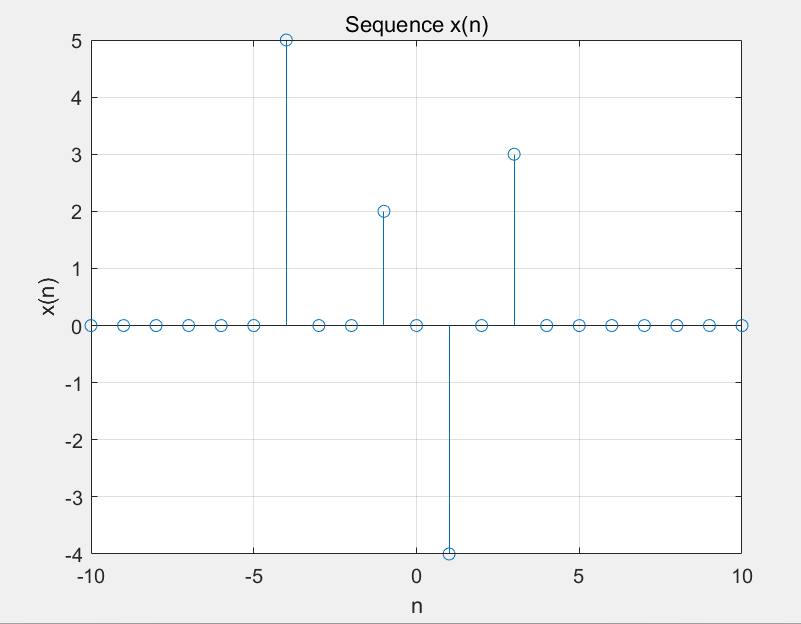
\includegraphics[scale=0.75]{22.png}
            \end{figure}
            \FloatBarrier
    \section*{23}
        \begin{lstlisting}[caption={题23 MATLAB代码}, label={lst:matlab}]
            % 定义序列参数
            alpha = 0.5;
            beta = 0.8;
            n0 = 0;
            N = 10;

            % 定义序列 h(n) 和 x(n)
            n_h = 0:N-1;
            h = alpha.^n_h;

            n_x = -10:10; % x(n)的范围根据实际情况调整
            x = zeros(size(n_x));
            x(n_x >= n0) = beta.^(n_x(n_x >= n0) - n0);

            % 计算卷积
            y = conv(h, x, 'same');

            % 调整卷积序列长度,使其与n_x相匹配
            n_y = n_x(1:length(y));

            % 绘制序列图形
            figure;
            subplot(3,1,1);
            stem(n_h, h, 'b', 'LineWidth', 1.5);
            xlabel('n');
            ylabel('h(n)');
            title('Sequence h(n)');

            subplot(3,1,2);
            stem(n_x, x, 'r', 'LineWidth', 1.5);
            xlabel('n');
            ylabel('x(n)');
            title('Sequence x(n)');

            subplot(3,1,3);
            stem(n_y, y, 'g', 'LineWidth', 1.5);
            xlabel('n');
            ylabel('y(n)');
            title('Convolution Sequence y(n)');


        \end{lstlisting}
        Answer: 
            \begin{figure}[h]
                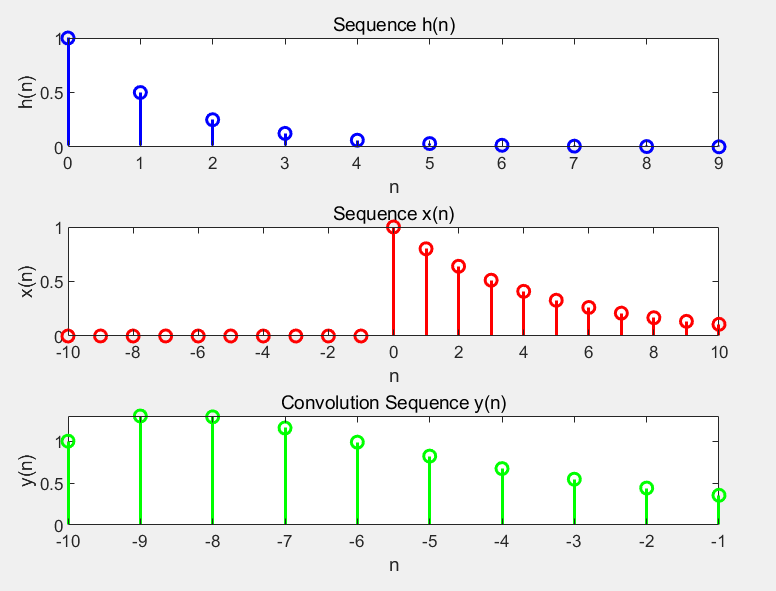
\includegraphics[scale=0.75]{23.png}
            \end{figure}
            \FloatBarrier
\end{document}